\begin{frame}{Le progrès de la science comme un processus \textit{discontinu}}
\begin{block}{Changement de paradigme}
Changement fondamental d'un paradigme à un autre, dans la façon dont les scientifiques abordent, pensent et comprennent un domaine donné.
\end{block}
Le nouveau \textit{paradigme}\footnote{Découvertes scientifiques universellement reconnues.} est incompatible avec le précédent.
\begin{itemize}
\item \og{}rupture entre observation et expérimentation\fg{} 
{\footnotesize(\cite{bachelard1934formation})}
\item \og{}révolution scientifique\fg{} {\footnotesize(\cite{koyre1957closed})}
\item \og{}changement de paradigme\fg{} {\footnotesize(\cite{kuhn1962structure})} 
\end{itemize} 
% start the columns environment
\begin{columns}[c]
% create the column with the text, that occupies  half of the slide
\begin{column}{.5\textwidth}
    
% wrap the text inside a block, so it looks better
    \begin{block}{Functions}
    The plot with teal color corresponds to the function $y=(x^3-1)^2$ and the plot with red color corresponds to the function $y=(x^{11}-1)^2$ 
    \end{block}
\end{column}
% create the column with the image, that also  occupies half of the slide
\begin{column}{.5\textwidth}
% command to actually insert the image
\centering
    \includegraphics[scale=0.2]{PlotFunctions.png}
\end{column}
\end{columns}.
%\begin{figure}
%    \centering
%    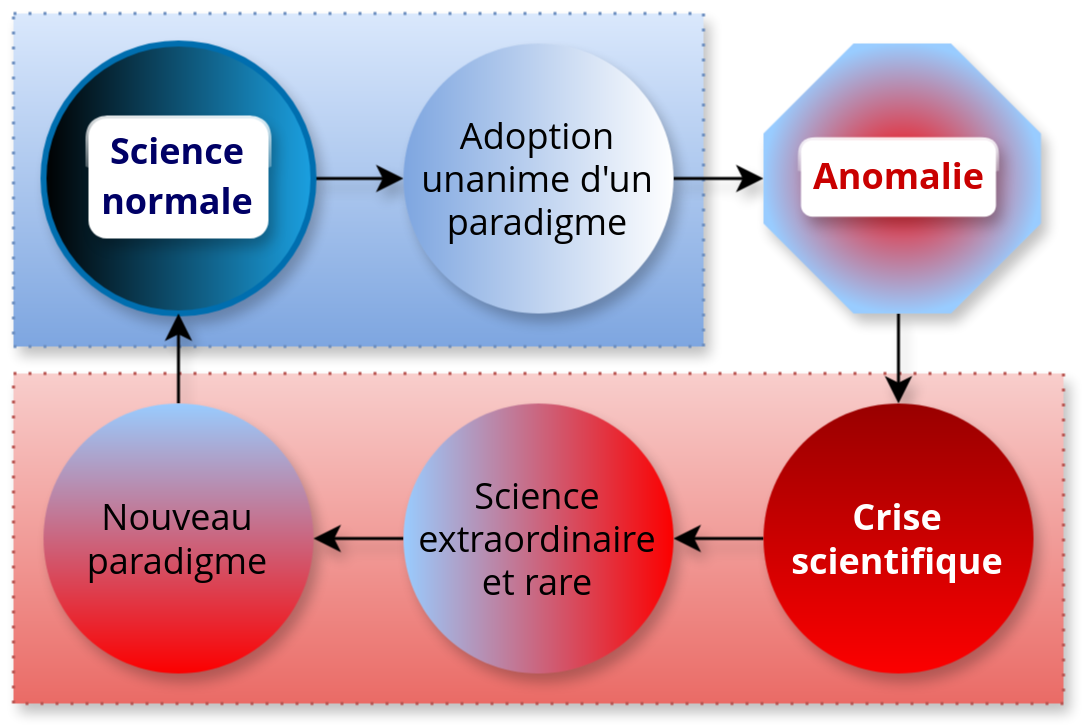
\includegraphics[width=65mm,scale=0.5]{pic/changement_paradigme.png}
%    \caption{Conception kuhnienne du progrès scientifique, adaptée de {\scriptsize\textcite{amiri}}.}
%    \label{fig:enter-label}
%\end{figure}
\end{frame}
